% Source: graduate-coursework/Research/Intro_to_Agents/handouts/Part5_TwoLayer_Agents.tex

\documentclass[border=4pt]{standalone}
\usepackage[T1]{fontenc}
\usepackage{graphicx}
\usepackage{lmodern}
\usepackage{tikz}
\usepackage{xcolor}
\usetikzlibrary{shapes.geometric, arrows.meta, positioning, fit, calc, backgrounds}

\definecolor{UofSCGarnet}{HTML}{73000a}
\definecolor{UofSCBlack}{HTML}{000000}
\definecolor{UofSCWhite}{HTML}{ffffff}
\definecolor{UofSCRose}{HTML}{CC2E40}
\definecolor{UofSCAtlantic}{HTML}{466A9F}
\definecolor{UofSCCongaree}{HTML}{1F414D}
\definecolor{UofSCHorseshoe}{HTML}{65780B}
\definecolor{UofSCGrass}{HTML}{CED318}
\definecolor{UofSCHoneycomb}{HTML}{A49137}
\definecolor{UofSC90Black}{HTML}{363636}
\definecolor{UofSC70Black}{HTML}{5C5C5C}
\definecolor{UofSC50Black}{HTML}{A2A2A2}
\definecolor{UofSCWarmGrey}{HTML}{676156}
\definecolor{UofSCSandstorm}{HTML}{FFF2E3}
\definecolor{UofSCDarkGarnet}{HTML}{570008}
\definecolor{UofSCAzalea}{HTML}{844247}

\tikzset{
    % Box styles - all sharp corners
    orchestrator/.style={
        rectangle,
        draw=UofSCGarnet,
        fill=UofSCGarnet!10,
        line width=1.5pt,
        minimum width=4cm,
        minimum height=1.2cm,
        align=center,
        font=\bfseries
    },
    worker/.style={
        rectangle,
        draw=UofSCAtlantic,
        fill=UofSCAtlantic!10,
        line width=1pt,
        minimum width=2cm,
        minimum height=0.9cm,
        align=center
    },
    task/.style={
        rectangle,
        draw=UofSCCongaree,
        fill=UofSCCongaree!10,
        line width=1pt,
        minimum width=1.8cm,
        minimum height=0.8cm,
        align=center
    },
    process/.style={
        rectangle,
        draw=UofSCBlack,
        fill=UofSCWhite,
        line width=1pt,
        minimum width=3cm,
        minimum height=0.8cm,
        align=center
    },
    result/.style={
        rectangle,
        draw=UofSCHorseshoe,
        fill=UofSCHorseshoe!10,
        line width=1pt,
        minimum width=2.5cm,
        minimum height=0.8cm,
        align=center
    },
    decision/.style={
        diamond,
        draw=UofSCGarnet,
        fill=UofSCGarnet!10,
        line width=1pt,
        minimum width=2cm,
        minimum height=1cm,
        align=center,
        aspect=2
    },
    % Arrow styles - straight lines only
    arrow/.style={
        ->,
        >=Stealth,
        line width=1pt,
        draw=UofSCBlack
    },
    thickarrow/.style={
        ->,
        >=Stealth,
        line width=1.5pt,
        draw=UofSCGarnet
    },
    dashedarrow/.style={
        ->,
        >=Stealth,
        line width=1pt,
        draw=UofSC70Black,
        dashed
    }
}

\begin{document}
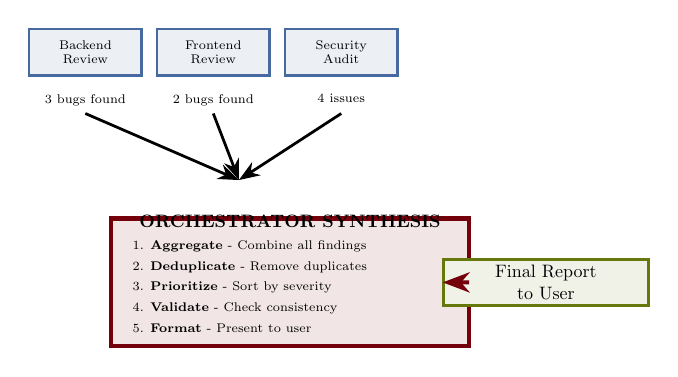
\begin{tikzpicture}[scale=0.65, transform shape]
    % Workers reporting
    \node[worker, minimum width=2.2cm, font=\scriptsize] (w1) at (-4,3) {Backend\\Review};
    \node[worker, minimum width=2.2cm, font=\scriptsize] (w2) at (-1.5,3) {Frontend\\Review};
    \node[worker, minimum width=2.2cm, font=\scriptsize] (w3) at (1,3) {Security\\Audit};

    % Results
    \node[font=\scriptsize, anchor=north] at (-4,2.3) {3 bugs found};
    \node[font=\scriptsize, anchor=north] at (-1.5,2.3) {2 bugs found};
    \node[font=\scriptsize, anchor=north] at (1,2.3) {4 issues};

    % Arrows to synthesis
    \draw[arrow] (-4,1.8) -- (-1,0.5);
    \draw[arrow] (-1.5,1.8) -- (-1,0.5);
    \draw[arrow] (1,1.8) -- (-1,0.5);

    % Synthesis box
    \node[orchestrator, minimum width=7cm, minimum height=2.5cm] (synth) at (0,-1.5) {};
    \node[font=\bfseries] at (0,-0.3) {ORCHESTRATOR SYNTHESIS};

    \node[font=\scriptsize, anchor=west] at (-3.2,-0.8) {1. \textbf{Aggregate} - Combine all findings};
    \node[font=\scriptsize, anchor=west] at (-3.2,-1.2) {2. \textbf{Deduplicate} - Remove duplicates};
    \node[font=\scriptsize, anchor=west] at (-3.2,-1.6) {3. \textbf{Prioritize} - Sort by severity};
    \node[font=\scriptsize, anchor=west] at (-3.2,-2.0) {4. \textbf{Validate} - Check consistency};
    \node[font=\scriptsize, anchor=west] at (-3.2,-2.4) {5. \textbf{Format} - Present to user};

    % Final output
    \node[result, minimum width=4cm] (out) at (5,-1.5) {Final Report\\to User};
    \draw[thickarrow] (3.5,-1.5) -- (out);
\end{tikzpicture}
\end{document}
